\documentclass[12pt]{article}
%\usepackage{caption}
\usepackage{setspace,graphicx,epstopdf,amsmath,amsfonts,amssymb,amsthm}
\usepackage{marginnote,datetime,enumitem,subfigure,rotating,fancyvrb}
\usepackage{hyperref,float}
\usepackage[longnamesfirst]{natbib}
\usepackage{mathtools}
\usepackage{caption}
\usepackage{float}
\usepackage{lscape}
\usepackage{graphicx}
\usepackage{flafter} 
\usepackage{tabularx} 
\usepackage{booktabs}
\usepackage{changepage}
\usepackage{setspace}
\usepackage{placeins}
\usepackage{threeparttable}
\usepackage{ragged2e}
\usepackage[export]{adjustbox}
\usepackage{stmaryrd}
\newcolumntype{Y}{>{\raggedleft\arraybackslash}X}% raggedleft column X
\usdate
\usepackage[a4paper,bindingoffset=0.2in,%
            left=0.8in,right=0.8in,top=1in,bottom=0.8in,%
            footskip=.35in]{geometry}



% SCRIPTS:
% use sp19_dailycimad_betas_10_upd for f1
% plan to use SP19_rm_34 to create all the tables with monthly returns

% Number paragraphs and subparagraphs and include them in TOC
\setcounter{tocdepth}{2}

% JF-specific includes:

\usepackage{indentfirst} % Indent first sentence of a new section.
\usepackage{endnotes}    % Use endnotes instead of footnotes


\begin{document}


\setlist{noitemsep}  % Reduce space between list items (itemize, enumerate, etc.)
\onehalfspacing      % Use 1.5 spacing
% Use endnotes instead of footnotes - redefine \footnote command
\renewcommand{\footnote}{\endnote}  % Endnotes instead of footnotes

\author{\large{Mykola Pinchuk}\thanks{\rm Simon Business School, University of Rochester. Email: Mykola.Pinchuk@ur.rochester.edu. \newline I would like to thank Alan Moreira, Yixin Chen, Shuaiyu Chen, Pingle Wang, Xuyanda Qi, David Swanson, Yushan Zhuang and Robert Mann for helpful comments. All errors are my own.}}

\title{\bf Cross-Industry Dispersion and the Cross-Section of Expected Returns}

\date{23 October 2019}  
% this is a version after Robert`s proofreading on 9/13/19, 3-4.20 pm.

\maketitle
\thispagestyle{empty}

\bigskip

\normalsize
\vspace{1cm}

\centerline{\bf Abstract}

\vspace{0.5cm}

\begin{onehalfspace}  % Double-space the abstract and don't indent it
  \noindent This paper examines cross-industry dispersion (CID), defined as a mean absolute deviation of returns of 49 industry portfolios. I find that expected stock returns are related cross-sectionally to the sensitivities of returns to innovations in CID. Annualized returns of the stocks with high sensitivity to CID are 8.2\% lower than the returns of the stocks with low sensitivity. Abnormal returns with respect to the best factor model are 5.8\%, suggesting that common factors can not explain this return spread. CID predicts unemployment, consistent with the hypothesis that CID is a proxy for unemployment risk from sectoral shifts. 
\end{onehalfspace}
\medskip


\clearpage
%\doublespacing
\setstretch{1.525}


\section{Introduction} \label{sec:Model}
The economy is a dynamic system with permanently evolving structure. As some industries are born, other industries lose their importance. Few people in 1970s could have predicted that within 20 years IT sector would capture the largest share of the stock market. There is no reason to expect a constant rate of this structural transformation. Naturally, accelerated structural transformation increases aggregate economic uncertainty and labor income risk for workers in underperforming industries. This paper explores the asset pricing implications of such sectoral reallocation and related labor risk.
\paragraph{}
The paper measures time-varying structural uncertainty using cross-industry dispersion (CID), defined as the mean absolute deviation of the returns of 49 industry portfolios. I document a novel evidence that stock exposures to cross-industry dispersion (CID) predict the cross section of expected returns. The paper finds that the firms with large return sensitivity to CID deliver smaller returns than the stocks with low sensitivity to CID. This finding suggests that in equilibrium there exists an extra demand for stocks, positively comoving with CID, implying low expected returns of these stocks. The long-short value-weighted portfolio, formed on the sensitivity to CID, delivers monthly return of 68 bps with abnormal returns of 48-79 bps. The results are not explained by the other measures of volatility and uncertainty. CID subsumes large fraction of cross-sectional return predictability of common idiosyncratic volatility CIV (Herskovic, Kelly, Lustig, van Niewerburgh 2016). 
\paragraph{}
This evidence is consistent with several broad sources of risk, possibly related to CID. Periods of highly nonhomogeneous performance of different industries (high CID) are likely to be periods of accelerated sectoral reallocation of resources and increased economic uncertainty. Times with a large wedge between winning and losing industries can proxy for the periods of rapid economic transformation, when some industries become more important, while the others lose relevance. High CID may indicate a temporary decrease in output and efficiency as resources are reallocated across sectors (Lilien 1982). 
\paragraph{}
More specifically, labor income risk can explain relevance of CID to asset pricing. By construction, high CID means that some industries severely underperform the market, while the others enjoy exceptionally high returns. This pattern is likely to raise a concern that losing industry is under the threat of dying. Naturally, this is a period of a negative shock to expected lifetime labor income of the employees in underperforming industries. The fact that there are both outperforming and underperforming industries with returns sufficiently far from the market return implies even larger labor income risk than the one during a recession. Within a recession, the common wisdom is that most of lost jobs will be recovered at some point in the future, while a disappearance of some industry means a loss of industry-specific jobs forever. 
\paragraph{}
While many occupations are demanded across industries, they are usually low skill occupations, less relevant to asset pricing. Losing high-wage job constitutes larger negative shock to lifetime income. Moreover, high-paid workers are likely to have more savings and produce larger effect on financial market. High-skill jobs (e.g., aerospace engineer) are usually confined to a few industries, implying very low across-industry labor mobility. Thus, I expect that CID captures the asset pricing effect of Cross-sectional Dispersion (CSD), consistent with labor income risk. According to labor income risk explanation, stocks with negative covariance with CID are more risky, since they tend to fall when the risk of losing high skill industry-immobile jobs is large.
\paragraph{}
This paper draws upon the theoretical contribution of Duffie and Constantinides (1996) to motivate CIV as a state variable. Duffie and Constantinides show that in a model with heterogeneous agents, subject to uninsurable labor income shocks, cross-sectional variance of agents' consumption growth becomes a state variable. As discussed above, severe underperformance of their industry suggests a negative shock to expected consumption growth of employees.
\paragraph{}
This article builds upon a body of work from macroeconomic literature. Lilien (1982) reports that sectoral shifts and performance dispersion result in unemployment shocks, caused by migration of employees between firms and sectors. Loungani, Rush and Tave (1990) construct stock market dispersion index and document that it predicts unemployment. Brainard and Cutler (1993) use similar measure to assess the contribution of sectoral reallocation to unemployment. They find that sectoral reallocation accounts for a large share of unemployment fluctuations at long horizons. Multiple studies (Summers and Carrol 1991, Blundell, Pistaferri and Preston 2008, Guvenen and Smith 2014, Heathcote, Storesletten and Violante 2014) document that households do not completely insure their consumption from persistent shocks to the labor income. These findings highlight the importance of labor income risk for asset pricing.
% lrt90 and bc93 used exactly the same cid and got the results. it seems that i already have at least some weak positive results, consistent with my labor story.
\paragraph{}
The research on economic uncertainty frequently uses cross-sectional dispersion of accounting variables as a measure of uncertainty. Bloom (2009) documents a strong correlation between the indicators of macroeconomic uncertainty, including time-series measures of market volatility, the cross-sectional variation of firms` pretax profit growth and returns as well as a dispersion across macroeconomic forecasts. He argues that all of these variables proxy for financial and macroeconomic uncertainty. Sadka (2012) finds that higher earnings dispersion is associated with higher expected returns, suggesting that earnings dispersion is a state variable, relevant for asset pricing. Jurado, Ludvigson and Ng (2015) use cross-sectional dispersion of a profit growth in order to construct the index of macroeconomic uncertainty.
\paragraph{}
This study contributes to several domains of literature. Different measures of market volatility have traditionally been used as a proxy for economic and financial uncertainty. Ang, Hodrick, Xing and Zhang (2006) empirically show that exposure of stocks to VIX is priced in the cross-section of expected stock returns. Herskovic, Kelly, Lustig and Van Nieuwerburgh (2016) report that stocks with larger sensitivity to common idiosyncratic volatility (CIV) earn lower expected returns. They argue that CIV proxies for idiosyncratic risk faced by households and suggest labor income risk as a main channel. Eiling (2013) uses industry-specific labor income growth rates to extend human capital CAPM (Jagannathan and Wang 1996) and shows that her empirical model can price 25 size and book-to-market portfolios. Eiling, Kan and Sharifkhani (2018) use production-based asset pricing model to justify the predictability of market returns by sectoral labor reallocation shocks. 
\paragraph{}
This paper is closely related to the literature on cross-sectional dispersion (CSD), defined as a standard (mean absolute) deviation of the cross section of stock returns. Bekaert and Harvey (1997, 2000) use CSD as a measure of development and maturity of the stock market. Stivers (2003, 2006, 2010) finds that CSD can predict idiosyncratic volatility as well as returns of value and momentum premia. Maio (2013, 2016) reports that the cross-sectional standard deviation of returns of the portfolios sorted on size and book-to-market can predict market returns. The closest paper to this one is Verousis and Voukelatos (2018). They find that the stocks with high sensitivity to CSD offer lower returns in their 1996-2012 sample. Due to the more idiosyncratic nature of CSD, the authors explain the findings by idiosyncratic risk without elaborating on or providing evidence for their explanation.
\paragraph{}
This paper uses 1963-2018 sample and shows that high sensitivities to CID predict lower expected returns. I argue that this predictability stems from return dispersion across industries, proxying for labor income risk due to sectoral shifts. These results suggest that only the across-industry component of CSD (i.e., CID) is priced. The long-short portfolio, formed on CID, controlling for CSD, delivers 35 bps (t-statistic=2.6) monthly abnormal returns, while the long-short portfolio, formed on CSD, controlling for CID, produces -5 bps returns. Therefore, these results suggest that cross-sectional predictability of returns by CSD is not driven by idiosyncratic risk, relevant for underdiverisified investors. CSD is a manifestation of more fundamental economic force - labor income risk from structural shifts, proxied by CID. 
\paragraph{}
Consistent with this explanation, high CID predicts high aggregate unemployment at a quarterly frequency. The results suggest that predictive power of CID for unemployment growth is driven by the long-term component of unemployment growth. Unlike aggregate demand shocks, sectoral reallocation shocks are likely to have permanent effect on unemployment growth (Brainard and Cutler 1993). Consistent with CID, proxying for labor income risk from sectoral shifts, CID strongly predicts long-term unemployment, but has little relationship with its short-term component.  Overall, these results support the explanation of CID premium by industry-specific human capital risk from sectoral shifts.

% there was the paper Jiang(2010), which seems totally retarded to me. the guy found 26% annualized quintile spread using beta from regression of returns on levels and explained it with the risk story with the wrong sign. do not want to cite it %.


\section{Data and Dispersion Measures} \label{sec:Model}

\subsection{Sample}

The paper uses stock price data from CRSP and accounting data from Compustat. The sample encompasses 1963-2018. I download macroeconomic data from St. Louis Federal Reserve Bank. 
I consider common stocks traded at NYSE, NASDAQ or AMEX and perform the main asset pricing tests at the monthly frequency. The sample of stock returns consists of 3107556 firm-month observations with nonmissing returns. In order to exclude small and illiquid stocks from the analysis, I restrict the sample to the stocks with price above \$10 and the stocks with market capitalization above \$10 million in 2018 dollars. After this restriction the sample consists of 1741865 firm-month observations. All the analysis below uses excess returns.
\paragraph{}
Kenneth French`s website is a source of data on stock market factors as well as industry classifications and returns of industry portfolios. I download uncertainty indices, constructed by Jurado, Ludvigson and Ng (2015) from Sydney Ludvigson`s website. 

\subsection{Construction of Dispersion Measures}

The paper defines cross-industry dispersion as the mean absolute deviation of returns across 49 industry portfolios at any given period.
\begin{equation}
CID_t = \frac{1}{N}\sum^{N}_{i=1}{|R_{it}-R_{MKT,t}|}.
\end{equation}
I use daily value-weighted returns of Fama-French 49 industry portfolios. I compute CID every day during the period, spanning 1927-2018. Since some industries have few firms at the beginning of the sample, the paper computes CID across the industries with at least 10 firms. I proxy for the market return with the value-weighted market return across all firms from CRSP (vwretd). I use the similar approach to calculate Cross-Sectional Dispersion (CSD) and Within-Industry Dispersion (WID).
\paragraph{}
The Figure 1 plots the time series of CID. Since the paper follows asset pricing literature and starts the sample of stock returns in 1963, I focus on CID after 1963. The time series of CID exhibits two large secular increases. The first long-term spike took place within 1998-2003 and is likely associated with the dotcom boom and the following decline. The second spike was recorded during 2007-2009, coinciding with the recent financial crisis. Both events are consistent with the hypothesis that CID proxies for some dimension of uncertainty and is related to the rate of sectoral shifts in the economy. Intuitively, CSD is a sum of CID and WID, so Figure 1 facilitates comparison between these variables. While before 2000, CSD was primarily driven by WID, during the recent two decades a relative importance of CID increased. This observation suggests increased comovement of returns within industries and a growing importance of classification of firms into industries.
\paragraph{}
The next step of the analysis will be to estimate sensitivities of the stocks to fluctuations in CID. To facilitate the interpretation of CID as a state variable from ICAPM (Merton 1973) and avoid econometric issues, I difference CID, using the same specification as in Pastor and Stambaugh (2003). That is, I calculate first difference of CID and estimate its residuals from AR(1) model:
\begin{equation}
\Delta(CID_t) = \gamma_0 + \gamma_1 \Delta(CID_{t-1}) + \gamma_2 CID_{t-1} + u_t.
\end{equation}
Abusing notation, I refer to the residual $\hat{u}_t$ as $CID_t$ in the rest of the paper. 1-lag autocorrelation of CID is -0.07, implying very low persistence. Thus, I can use $CID_t$ as an explanatory variable in predictive regressions without spurious regression issues (Novy-Marx 2013). 
\paragraph{}
Table 1 reports correlations of CID with other measures of uncertainty and volatility. Since all time series are differenced according to Pastor and Stambaugh (2003) specification, the correlations are relatively low. CID has positive correlation with all the variables, ranging from 0.06 to 0.33. The results suggest that CID is distinct from, though positively related to frequently used uncertainty and volatility measures.

\section{Asset Pricing Results} \label{sec:Model}

This section documents and discusses the main results of the paper. First, I explain how I estimate the sensitivity of stock returns to CID. Then, I form decile portfolios on $\beta_{CID}$ and compute their returns. Finally, the section discusses the asset pricing performance of different measures of cross-sectional dispersion.

\subsection{Estimation of $\beta_{CID}$}
I use daily stocks returns in order to obtain precise estimates of their sensitivities to CID. The paper uses two years of daily excess returns to estimate betas from the following time series regression:
\begin{equation}
R_{it}=\alpha+\beta CID_t + \epsilon_t.
\end{equation}
Since controlling for market returns has little effect on the results, I use simpler specification (3). I estimate betas over the period 1963-2018. To compensate for the extreme values of $\hat{\beta}_{CID}$, possibly resulting from imprecise estimation, I winsorize $\hat{\beta}_{CID}$ at 1\% and 99\% percentiles. Section 5.4 verifies that the results are not due to factors, omitted during estimation of $\beta_{CID}$.  

\subsection{Portfolios, formed on $\beta_{CID}$}

In the remainder of this section, the paper uses the monthly frequency. Every month, I sort the stocks into decile portfolios based on their $\beta_{CID}$. I update estimates of $\beta_{CID}$ and rebalance portfolios every month. To calculate post-ranking betas, I run the  regression above for each decile portfolio using the full sample. Figure 2 plots post-ranking betas against pre-ranking betas. Not surprisingly, the spread decreases from 3.2 in pre-ranking betas to 0.6 in post-ranking betas. Clearly monotonic and almost linear relationship between post-ranking and pre-ranking betas suggests that pre-ranking betas are reasonably good estimates of post-ranking betas. Due to noise in estimation, we expect that post-ranking $\beta_{CID}$ will shrink towards $\beta_{CID}$ of the market. Full-sample $\beta^{MKT}_{CID}$ is 0.29, explaining why post-ranking betas range between 0 and 0.6.
\paragraph{}
Table 2 reports mean values of characteristics of decile $\beta_{CID}$-sorted value-weighted portfolios. Stocks in the highest decile are larger, more profitable, more liquid, have slower asset growth and lower past returns. Table 3 describes excess returns of equally-weighted and value-weighted portfolios, formed on $\beta_{CID}$. The equally-weighted long-short portfolio has average returns of 90 bps, though this spread is mostly driven by the returns of the first decile. Returns of value-weighted portfolios, sorted on $\beta_{CID}$, decrease almost monotonically. The long-short value-weighted portfolio generates 68 bps average monthly returns with t-statistic of 3.8. 
\paragraph{}
Table 4 presents abnormal returns of the value-weighted decile portfolio with respect to most frequently used factor models. Controlling for Fama-French 5 factors does not have significant effect on the CID premium. T-statistic of these abnormal returns stays comfortably below -3, meeting the challenge of Harvey et al. (2016). Fama-French 5 factor model, augmented with momentum and short-term reversal factors, somewhat decreases abnormal returns to 48 bps (t-statistics = -2.9). While the loadings on size, momentum and short-term reversal factors can explain a fraction of returns of this trading strategy, the loadings on market and value factors make these returns even more anomalous (Table 5).
\paragraph{}
Table 6 reports the returns of long-short portfolios, double-sorted on size and CID. Even controlling for size, the long-short portfolio from tercile sorts on CID delivers statistically significant abnormal returns of 23-31 bps. Controlling for momentum factor decreases the abnormal returns to 15-16 bps. The weaker results are likely driven by both size effect and a low precision of $\beta_{CID}$ estimates, combined with very coarse sorts.

\subsection{Cross-sectional Results}

To check a robustness of the cross-sectional predictability of returns by $\beta_{CID}$, I employ Fama-MacBeth regressions. Table 7 reports that $\beta_{CID}$ is a significant determinant of excess returns (t-statistic above 2.4). Consistent with the previous findings, the results weaken after controlling for size. An increase in $\beta_{CID}$ by 1 unit is related to 1.13\% lower excess returns. Since the standard deviation of $\beta_{CID}$ is 1.00, the results suggest that 1 standard deviation increase in $\beta_{CID}$ is associated with 1.13\% smaller returns. Therefore, the estimated price of CID risk is 1.13\%. Small economic magnitude of this number can be a result of the estimation, based on linear regression, capturing only linear relationship. Nonparametric results above suggest larger magnitude of CID risk premium.

\subsection{Performance of different dispersion measures}

Verousis and Voukelatos (2018) find that in 1996-2012 sample lower CSD is associated with high excess returns. The obvious question is whether CSD premium is driven by its across-industry component (CID) or within-industry component (WID). To answer this question, I perform double sorts on WID and CID. Table 8 reports the results with value-weighted portfolios from 5x5 double sorts. I construct the long-short portfolio from the sort on CID, controlling for WID, and vice versa. The long-short portfolio from WID sorts delivers abnormal returns between 25 and -16 bps, not significantly different from zero. The long-short portfolio from CID sorts produces abnormal returns between 28 and 53 bps, which are highly significant. These results clearly imply that unlike WID, CID captures a priced dimension of cross-sectional dispersion. 
\paragraph{}
Table 9 reports the similar results from 5x5 double sorts on $\beta_{CID}$ and $\beta_{CSD}$. The long-short portfolio from CSD sorts produces significantly negative abnormal returns with respect to Fama-French 5 factor model, augmented with momentum factors. Since these returns have the sign, inconsistent with the idiosyncratic risk explanation of Verousis and Voukelatos, the results clearly suggest that CSD predicts the cross section of expected returns only through CID. Controlling for CSD, CID long-short portfolio generates abnormal returns between 17 and 35 bps. Overall, the results suggest that CID reflects a priced component of cross-sectional volatility.

\section{Economic Channel: Labor Income Risk} \label{sec:Model}

\subsection{Economic Mechanism}

Constantinides and Duffie (1996) develop the model with agents, subject to heterogeneous uninsurable income shocks. They show that the cross-sectional variance of individual consumption growth enters Euler equation. While the model analytically proves the relevance of the cross-sectional variance of consumption growth for asset pricing, it remains silent on its economic channels and meaning. This story naturally fits macrolabor literature which uses different measures of dispersion of stock returns to assess unemployment shocks, resulting from structural shifts.
\paragraph{}
Fluctuations in individual labor income can arise from two channels: a change in wage and a change in employment. Larger magnitude of labor income shocks from employment loss as well as downward wage rigidity suggests that unemployment risk is the most important component of labor income fluctuations for asset pricing. Macroeconomic literature views the changes in aggregate employment as the result of two forces: aggregate shocks and reallocation shocks. Lilien (1982) introduces the sectoral shifts hypothesis entailing that higher dispersion of intersectoral shifts leads to higher unemployment by increasing amount of labor reallocation. While Lilien uses the variance of employment growth across sectors to measure the reallocation, Loungani, Rush and Tave (1990) argue that the variance of stock returns across sectors is more precise and forward-looking measure. 
\paragraph{}
This paper uses CID to capture a divergence in performance across industries, indicative of a change in sectoral composition of the economy. Therefore, periods of high CID are indicators of increased risk of losing lobs in underperforming industries. While many occupations are not industry-specific (e.g., janitor), the others are closely related to few industries (e.g., aerospace engineer). A potential disappearance of underperforming industry constitutes large labor income risk for such high-skill industry-specific occupations. Addison and Portugal (1989) as well as Jacobson, LaLonde and Sullivan (1993) document that workers experience large wage decrease after switching industry. 
\paragraph{}
According to this story, changes in CID should have positive relationship with both contemporaneous and future unemployment growth. Since a positive shock to CID reflects an increase in the rate of sectoral reallocation of resources and labor, it should be associated with layoffs. Therefore, we expect a positive relationship between CID changes and unemployment changes. Since stock prices have more forward-looking nature and move faster than measures of real economic activity, the firm's employment decision will respond to stock returns with some lag. Thus, we expect positive predictability of unemployment growth by CID changes.

\subsection{Results}

Table 11 shows that CID predicts unemployment at the quarterly frequency, controlling for other stock market-based predictors of business cycles.
Using the sample of 1948-2019, I regress unemployment growth at the changes in CID in the previous quarter. The first two columns report positive and statistically significant coefficients (t-statistic of 2.72 and 2.53), suggesting that the results are robust to known stock market predictors of business cycle. These results are consistent with the findings of Loungani, Rush, Tave (1990) and Brainard, Cutler (1993) and suggest that CID can forecast unemployment growth. 
\paragraph{}
Labor risk explanation of CID premium is based on the idea that CID reflects more permanent component of unemployment risk, arising from sectoral shifts as opposed to aggregate shocks. Macroeconomic literature argued that while unemployment from aggregate shocks have transitory nature, sectoral shifts have more long-term effects on unemployment. For example, if small short-term aggregate shock hits the economy, then struggling firms in different industries are likely to fire workers to cut the costs. As long as there are no industries, disproportionally affected by this shock, it will not cause sectoral reallocation of labor. Successful firms are likely to hire workers, fired from struggling firms in the same industries. Therefore, such short-term aggregate shocks are unlikely to have a major effect on long-term unemployment.
\paragraph{}
The last four columns of Table 11 show that the predictability of unemployment growth by CID changes is mostly driven by long-term component of unemployment growth. CID predicts growth in long-term unemployment (t-statistics 2.04), but can not predict growth in short-term unemployment. Adjusted $R^2$ of these regressions provide even stronger results. While CID explains 3\% of the variation in future long-term unemployment growth, adding aggregate market predictors (first and second moments of market returns) increases this fraction to 5\%. On the other hand, CID has no explanatory power for the variation in future short-term unemployment growth  as evidenced by negative adjusted $R^2$. However, adding aggregate market controls increases the fraction of explained variation to 11\%. These results suggest that CID is more important predictor of long-term unemployment than aggregate stock market variables are, while these aggregate variables are much better predictors of short-term unemployment growth. These findings are consistent with CID reflecting sectoral shifts and aggregate stock market variables accounting for aggregate short-term shocks. Thus, the evidence supports the explanation of CID premium by long-term unemployment risk from sectoral shifts.

\subsection{Future work}

To provide the evidence on the relationship between CID and unemployment risk from sectoral shifts, I intend to check whether CID predicts the dispersion in employment growth across sectors.
\paragraph{}
Fama-French industry classification is based on the product market, so it is not a perfect measure for CID premium, hypothetically driven by labor income risk. Therefore in the later versions of the paper I will attempt to use/construct industry classifications, based on labor market competition and a type of workers` human capital. One possible solution is to use BLS OES (Occupational Employment Statistics) data to construct occupation-based industry classification. Alternatively, I can look at text-based network industry classification of Hoberg and Philips (2016).


\section{Further results} \label{sec:Model}
\subsection{Robustness to different industry definitions}

Since Fama-French (FF) 49 industry classification is arbitrary, I explore the robustness of the findings to industry definitions at the varying levels of coarseness. I compute CID using FF30, FF17, FF10 and FF5 industry definitions. Figure 4 reports CID premium at the different levels of industry aggregation. The results change a little as industry coarseness increases. Surprisingly, we observe large CID premium even as the paper computes CID across 5 industry portfolios. The results suggest that CID premium reflects the variation of returns between few broad industries.  

\subsection{Robustness to other uncertainty measures}

Table 1 reports the correlations between CID and other measures of uncertainty: VIX, market volatility, financial uncertainty (Jurado, Ludvigson and Ng 2015), macroeconomic uncertainty (Jurado, Ludvigson and Ng 2015) and common idiosyncratic volatility (Herskovic, Kelly, Lustig and Van Nieuwerburgh 2016). Consistent with the hypothesis that all these variables capture financial uncertainty, CID has a positive correlations with all of them. On the other hand, the largest correlation of CID with these variables is 30\%, implying that CID is not just a noisy proxy for these uncertainty measures.
\paragraph{}
Table 10 reports the relationship between CID premium and aforementioned uncertainty variables. I use 5x5 double sorts to control for sensitivities to these uncertainty measures. Double sorts on $\beta_{CID}$ and $\beta_{Vol}$ indicate that both variables are associated with large risk premium, robust to controlling for asset pricing factors. The long-short portfolio, constructed on $\beta_{CID}$ sorts, produces abnormal returns between 32 and 48 bps and t-statistics above 2.7. Panels C and D show that $\beta_{CID}$ subsumes the relationship between stock sensitivities to financial and macroeconomic uncertainty (Ludvigson 2015) and expected returns. 
% need to read that paper, because i am not sure that they claim that.
The Panel B suggests that $\beta_{CID}$ outperforms $\beta_{CIV}$. Abnormal returns of $\beta_{CID}$-based long-short portfolio range between 26 and 44 bps versus 8 and 27 bps for $\beta_{CIV}$-based long-short portfolio. $\beta_{VIX}$ is the only variable, controlling for which eliminates statistical significance of the CID premium. Controlling for VIX exposure, long-short portfolios, formed on $\beta_{CID}$, deliver 15-38 bps abnormal returns. Since these returns are economically significant and a loss of statistical significance appears to be driven by less precise estimates, I would hesitate to say that VIX exposure explains CID premium.

\subsection{Results at lower frequency}

Risk-based explanation of CID premium entails that the investors, more exposed to labor income risk from sectoral shifts, should buy high $\beta_{CID}$ stocks. It is not immediately clear that economic agents are sensitive to changes in labor income risk at the monthly frequency. Therefore, I verify the existence of the CID premium at lower frequencies.
\paragraph{}
Panel A of Table 12 shows that the value-weighted long-short decile portfolio, formed on $\beta_{CID}$, delivers 115 bps of quarterly returns. Abnormal returns range between 73 and 193 bps. Panel B of Table 12 reports that the value-weighted long-short decile portfolio, formed on $\beta_{CID}$, produces 208 bps of semiannual returns. Abnormal semiannual returns are between 128 and 333 bps. While these returns are smaller in annualized magnitude than annualized monthly returns, they show the same statistically significant pattern. Panel C of Table 12 presents annual returns of the value-weighted long-short decile portfolio, formed on $\beta_{CID}$. It generates 6.82\% of unconditional returns and alpha between 1.97\% and 8.04\%. While abnormal returns with respect to Carhart and FF5+Mom+STR lose statistical significance, it is likely driven by the decreased statistical power from fewer observations. Overall, the results suggest that the CID premium exists at any frequency between the monthly and the annual frequency and is not explained by common asset pricing factors.

\subsection{Common factors in industry portfolios}

One possible explanation of documented results is the difference in loadings on common factors across industries. According to this hypothesis, the time-series variation in CID merely reflects the variation in asset pricing factors. For example, if there is a large heterogeneity in loadings on the profitability factor across industries, then periods of very large or very low returns of the RMW factor will mechanically generate large CID.
\paragraph{}
To test this explanation, I use abnormal returns of industry portfolios with respect to Fama-French 5 factor model to calculate CID. Tables 13 reports that hedging factor exposures has no effect on decile returns. Furthermore, Table 14 suggests that controlling for factor loadings across industries increases a magnitude of abnormal returns. Abnormal returns with respect to the best factor model are 58 bps (t-stat = -3.35). 

%\newpage
\vspace{1cm}

\section{Conclusion} \label{sec:Model}

This paper introduces CID as a measure of labor income risk from sectoral shifts and explores its asset pricing implications. Stocks with low $\beta_{CID}$ are more risky, since they decline precisely when investors are subject to increased labor income risk. Consistent with this idea, these stocks produce higher returns. The value-weighted long-short portfolio, formed on $\beta_{CID}$, delivers 68 bps monthly returns. Abnormal returns range between 48 and 79 bps. A heterogeneity in factor loadings across industry portfolios does not explain these findings. The results are not explained by known measures of uncertainty and labor income risk, such as VIX (Ang, Hodrick, Xing and Zhang 2006), macroecocnomic and financial uncertainty (Jurado, Ludvigson and Ng 2015) or common idiosyncratic volatility (Herskovic, Kelly, Lustig and Van Nieuwerburgh 2016). I show that the previously documented cross-sectional predictability of returns by cross-sectional dispersion (CSD, Verousis and Voukelatos 2018) is a manifestation of the CID premium. Controlling for CID, CSD loses its asset pricing relevance, implying that CID reflects a priced component of CSD.
\paragraph{}
These findings are consistent with the hypothesis that CID premium arises due to labor income risk from sectoral shifts. This paper uses CID as a proxy for a rate of sectoral shifts, leading to unemployment risk in underperforming industries. Consistent with macroeconomic literature, I find that CID predicts unemployment. This predictability is mostly driven by medium-term and long-term unemployment, in line with more permanent effect of sectoral reallocation shocks on unemployment. These results support the idea that CID premium is driven by industry-specific human capital risk due to sectoral shifts.


\newpage
\section{References:}
\begin{enumerate}

    \item{Addison, John T., and Pedro Portugal. "Job displacement, relative wage changes, and duration of unemployment." Journal of Labor economics 7, no. 3 (1989): 281-302.}
    \item{Ang, Andrew, Robert J. Hodrick, Yuhang Xing, and Xiaoyan Zhang. "The cross‐section of volatility and expected returns." The Journal of Finance 61, no. 1 (2006): 259-299.}
    \item{Black, Fischer. "Noise." The journal of finance 41, no. 3 (1986): 528-543.}
    \item{Becker, Gary S. "Investment in human capital: A theoretical analysis." Journal of political economy 70, no. 5, Part 2 (1962): 9-49.}
    \item{Bekaert, Geert, and Campbell R. Harvey. "Emerging equity market volatility." Journal of Financial economics 43, no. 1 (1997): 29-77.}
    \item{Bekaert, Geert, and Campbell R. Harvey. "Foreign speculators and emerging equity markets." The Journal of Finance 55, no. 2 (2000): 565-613.}
    \item{Bloom, Nicholas. "The impact of uncertainty shocks." econometrica 77, no. 3 (2009): 623-685.}
    \item{Blundell, Richard, Luigi Pistaferri, and Ian Preston. "Consumption inequality and partial insurance." American Economic Review 98, no. 5 (2008): 1887-1921.}
    \item{Brainard, S. Lael, and David M. Cutler. "Sectoral shifts and cyclical unemployment reconsidered." The Quarterly Journal of Economics 108, no. 1 (1993): 219-243.}
    \item{Carroll, Christopher D., and Lawrence H. Summers. "Consumption growth parallels income growth: some new evidence." In National saving and economic performance, pp. 305-348. University of Chicago Press, 1991.}
    \item{Connolly, Robert, and Chris Stivers. "Momentum and reversals in equity‐index returns during periods of abnormal turnover and return dispersion." The Journal of Finance 58, no. 4 (2003): 1521-1556.}
    \item{Connolly, Robert, and Chris Stivers. "Information content and other characteristics of the daily cross-sectional dispersion in stock returns." Journal of Empirical Finance 13, no. 1 (2006): 79-112.}
    \item{Constantinides, George M., and Darrell Duffie. "Asset pricing with heterogeneous consumers." Journal of Political economy 104, no. 2 (1996): 219-240.}
    \item{Eiling, Esther. "Industry‐specific human capital, idiosyncratic risk, and the cross‐section of expected stock returns." The Journal of Finance 68, no. 1 (2013): 43-84.}
    \item{Eiling, Esther, Raymond Kan, and Ali Sharifkhani. "Sectoral labor reallocation and return predictability." Rotman School of Management Working Paper 2602215 (2018).}
    \item {Fama, Eugene F., and James D. MacBeth. "Risk, return, and equilibrium: Empirical tests." Journal of political economy 81, no. 3 (1973): 607-636.}
    \item {Fama, E. F., \& French, K. R. (2015). A five-factor asset pricing model. Journal of Financial Economics, 116(1), 1–22. }
    \item{Goyal, Amit, and Pedro Santa‐Clara. "Idiosyncratic risk matters!." The Journal of Finance 58, no. 3 (2003): 975-1007.}
    \item{Guvenen, Fatih, and Anthony A. Smith. "Inferring labor income risk and partial insurance from economic choices." Econometrica 82, no. 6 (2014): 2085-2129.}
    \item {Harvey, Campbell R., Yan Liu, and Heqing Zhu. "… and the cross-section of expected returns." The Review of Financial Studies 29, no. 1 (2016): 5-68.}
    \item{Heathcote, Jonathan, Kjetil Storesletten, and Giovanni L. Violante. "Consumption and labor supply with partial insurance: An analytical framework." American Economic Review 104, no. 7 (2014): 2075-2126.}
    \item{Herskovic, Bernard, Bryan Kelly, Hanno Lustig, and Stijn Van Nieuwerburgh. "The common factor in idiosyncratic volatility: Quantitative asset pricing implications." Journal of Financial Economics 119, no. 2 (2016): 249-283.}
    \item{Hoberg, Gerard, and Gordon Phillips. "Text-based network industries and endogenous product differentiation." Journal of Political Economy 124, no. 5 (2016): 1423-1465.}
    \item{Jagannathan, Ravi, and Zhenyu Wang. "The conditional CAPM and the cross‐section of expected returns." The Journal of finance 51, no. 1 (1996): 3-53.}
    \item{Jacobson, Louis S., Robert J. LaLonde, and Daniel G. Sullivan. "Earnings losses of displaced workers." The American economic review (1993): 685-709.}
    \item {Jensen, Michael C., Fischer Black, and Myron S. Scholes. "The capital asset pricing model: Some empirical tests." (1972).}
    \item{Jorgensen, Bjorn, Jing Li, and Gil Sadka. "Earnings dispersion and aggregate stock returns." Journal of Accounting and Economics 53, no. 1-2 (2012): 1-20.}
    \item{Jurado, Kyle, Sydney C. Ludvigson, and Serena Ng. "Measuring uncertainty." American Economic Review 105, no. 3 (2015): 1177-1216.}
    \item{Lilien, David M. "Sectoral shifts and cyclical unemployment." Journal of political economy 90, no. 4 (1982): 777-793.}
    \item{Loungani, Prakash, Mark Rush, and William Tave. "Stock market dispersion and unemployment." Journal of Monetary Economics 25, no. 3 (1990): 367-388.}
    \item{Maio, Paulo F. "Return dispersion and the predictability of stock returns." Available at SSRN 1986791 (2013).}
    \item{Maio, Paulo. "Cross-sectional return dispersion and the equity premium." Journal of Financial Markets 29 (2016): 87-109.}
    \item{Merton, Robert C. "An intertemporal capital asset pricing model." Econometrica 41, no. 5 (1973): 867-887.}
    \item{Novy-Marx, Robert. "Predicting anomaly performance with politics, the weather, global warming, sunspots, and the stars." Journal of Financial Economics 112, no. 2 (2014): 137-146.}
    \item{Pastor, Lubos, and Robert F. Stambaugh. "Liquidity risk and expected stock returns." Journal of Political economy 111, no. 3 (2003): 642-685.}
    \item{Stivers, Chris, and Licheng Sun. "Cross-sectional return dispersion and time variation in value and momentum premiums." Journal of Financial and Quantitative Analysis 45, no. 4 (2010): 987-1014.}
    \item{Verousis, Thanos, and Nikolaos Voukelatos. "Cross-sectional dispersion and expected returns." Quantitative finance 18, no. 5 (2018): 813-826.}

\end{enumerate}

\newpage


\newgeometry{left=2.5cm, right=0.75cm, top=1.75cm, bottom=1.25cm}
\section*{Appendix}


\begin{figure}[h!]
\textbf{Figure 1: Dispersion Measures}
\vskip 6 pt
\begin{flushleft}
{The plot describes the time series of cross-industry dispersion (CID) and within-industry dispersion (WID). All the measures are calculated as the mean absolute deviation of returns at the daily frequency. Industries are defined according to Fama-French 49 industry classification. The paper uses value-weighted industry returns to calculate CID.}
\end{flushleft}
\centering
\vspace{0.64cm}
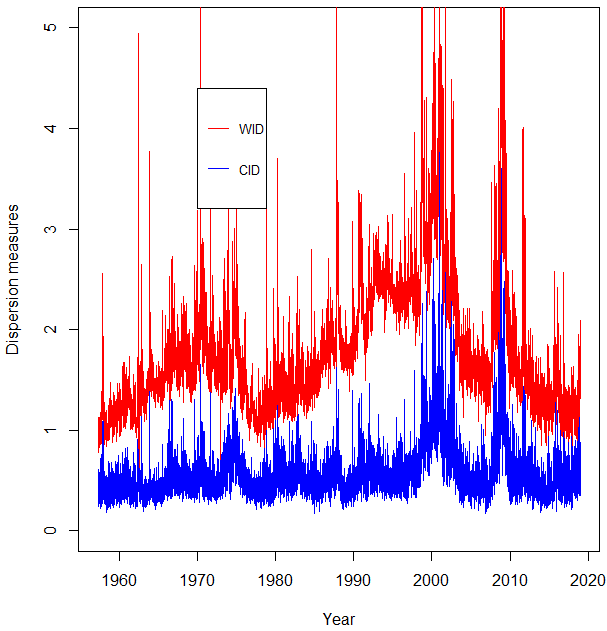
\includegraphics[width=0.9\textwidth]{paper_b2/Figure1.png}
\end{figure}

\begin{figure*}
\textbf{Figure 2: Postranking $\beta_{CID}$}
\vskip 12 pt
\begin{flushleft}
{The plot describes the relationship between postranking and preranking $\beta_{CID}$ of decile portfolios, sorted on $\beta_{CID}$. Preranking betas are estimated from regression (3) using 504 most recent days. To calculate postranking betas, I run the  regression (3) for each decile portfolio.}
\end{flushleft}
\centering
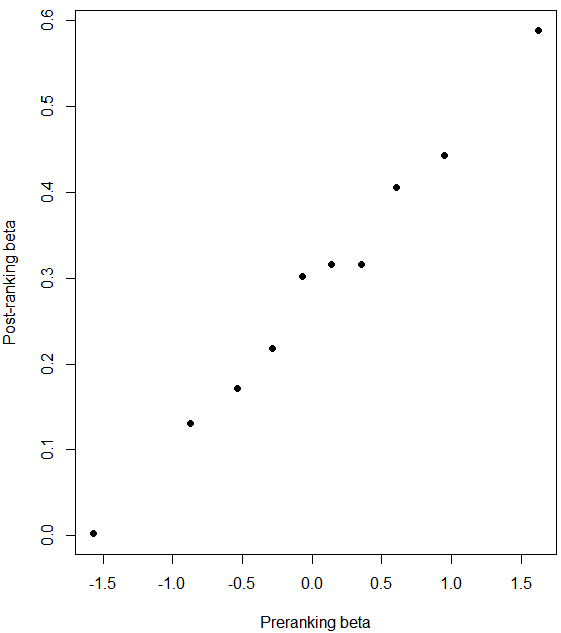
\includegraphics[width=1\textwidth]{fig2.png}
\end{figure*}


\begin{figure*}
\textbf{Figure 3: Performance of \$1 (log scale)}
\vskip 12 pt
\begin{flushleft}
{The plot describes the growth of \$1, invested in the long-short unisorted decile value-weighted portfolio, formed on $\beta_{CID}$.}
\end{flushleft}
\centering
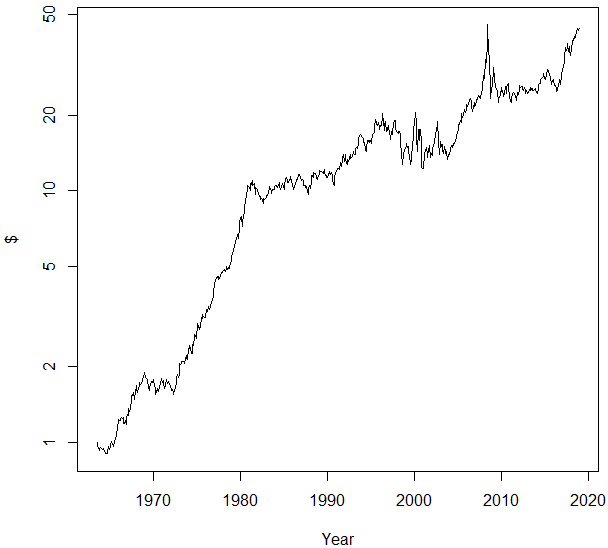
\includegraphics[width=1\textwidth]{Figure3.png}
\end{figure*}


\begin{figure*}
\textbf{Figure 4: Returns of decile L/S portfolio using different Fama-French industry partitions}
\vskip 12 pt
\begin{flushleft}
{The plot describes monthly returns and abnormal returns of decile L/S portfolios, formed on $\beta_{CID}$. I use Fama-French industry definitions with different coarseness: 49, 30, 17, 10 and 5 industries to compute CID. Abnormal returns are calculated with respect to Fama-French 5 factor model, including Momentum and Short-term Reversal factors.}
\end{flushleft}
\centering
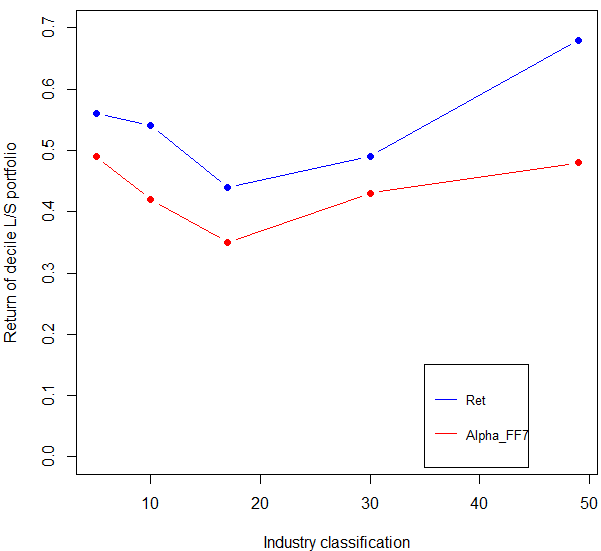
\includegraphics[width=1\textwidth]{paper_b2/Figure4.png}
\end{figure*}


\clearpage


% Table created by stargazer v.5.2.2 by Marek Hlavac, Harvard University. E-mail: hlavac at fas.harvard.edu
% Date and time: Tue, Sep 03, 2019 - 1:38:31 PM
\begin{table}[!htbp] \centering 
  \caption{\textbf{Correlations of changes in CID with changes of other variables}} 
  \label{} 
    \begin{flushleft}
    {\medskip\small
 The table reports correlations between changes in CID and changes in other variables at the monthly frequency. VIX is implied volatility, available starting from 1990. FU and MU are financial and macroeconomic uncertainty from Sydney Ludvigson website. VOL is the volatility of monthly value-weighted market index over the recent 24 months. CIV is common idosyncratic volatility (Kelly et al., 2016). }
    \medskip
    \end{flushleft}
\begin{tabular}{@{\extracolsep{5pt}} ccccccc} 
\\[-1.8ex]\hline 
\hline \\[-1.8ex] 
 & VIX & FU & MU & VOL & CIV & CID \\ 
\hline \\[-1.8ex] 
VIX & $1$ & $0.40$ & $0.36$ & $0.34$ & $0.50$ & $0.19$ \\ 
FU & $0.40$ & $1$ & $0.44$ & $0.30$ & $0.39$ & $0.10$ \\ 
MU & $0.36$ & $0.44$ & $1$ & $0.11$ & $0.24$ & $0.06$ \\ 
VOL & $0.34$ & $0.30$ & $0.11$ & $1$ & $0.27$ & $0.33$ \\ 
CIV & $0.50$ & $0.39$ & $0.24$ & $0.27$ & $1$ & $0.28$ \\ 
CID & $0.19$ & $0.10$ & $0.06$ & $0.33$ & $0.28$ & $1$ \\ 
\hline \\[-1.8ex] 
\end{tabular} 
\end{table}

\vspace{2cm}

% Table created by stargazer v.5.2.2 by Marek Hlavac, Harvard University. E-mail: hlavac at fas.harvard.edu
% Date and time: Tue, Sep 03, 2019 - 1:39:07 PM
\begin{table}[!htbp] \centering 
  \caption{\textbf{Characteristics of decile $\beta_{CID}$-sorted vw portfolios}} 
  \label{} 
    \begin{flushleft}
    {\medskip\small
 The table reports mean values of characteristics of decile portfolios, sorted on $\beta_{CID}$. Size is log of market equity in the previous month. Bm is log of Book-to-Market. Op is operating profitability. BAspr is the average bid-ask spread as a percentage of average price over the previous month. }
    \medskip
    \end{flushleft}
\begin{tabular}{@{\extracolsep{0pt}} lccccccccccc} 
\\[-1.8ex]\hline 
\hline \\[-1.8ex] 
 & D1 & D2 & D3 & D4 & D5 & D6 & D7 & D8 & D9 & D10 & LS \\ 
\hline \\[-1.8ex] 
RET & $1.16$ & $0.88$ & $0.85$ & $0.73$ & $0.63$ & $0.66$ & $0.66$ & $0.61$ & $0.54$ & $0.49$ & $$-$0.68$ \\ 
RET\_tstat & $4.87$ & $4.52$ & $4.64$ & $4.15$ & $3.82$ & $4.04$ & $3.89$ & $3.61$ & $2.98$ & $2.24$ & $$-$3.82$ \\ 
prebeta & $$-$1.57$ & $$-$0.87$ & $$-$0.54$ & $$-$0.29$ & $$-$0.07$ & $0.14$ & $0.35$ & $0.60$ & $0.95$ & $1.63$ & $3.20$ \\ 
postbeta & $0.002$ & $0.13$ & $0.17$ & $0.22$ & $0.30$ & $0.32$ & $0.32$ & $0.41$ & $0.44$ & $0.59$ & $0.60$ \\ 
size & $6.99$ & $7.58$ & $7.91$ & $8.19$ & $8.38$ & $8.61$ & $8.78$ & $8.92$ & $9.04$ & $8.88$ & $1.89$ \\ 
bm & $$-$0.83$ & $$-$0.76$ & $$-$0.76$ & $$-$0.73$ & $$-$0.73$ & $$-$0.74$ & $$-$0.74$ & $$-$0.77$ & $$-$0.83$ & $$-$0.86$ & $$-$0.03$ \\ 
op & $0.15$ & $0.16$ & $0.17$ & $0.17$ & $0.17$ & $0.17$ & $0.17$ & $0.17$ & $0.17$ & $0.17$ & $0.02$ \\ 
inv & $0.29$ & $0.22$ & $0.17$ & $0.16$ & $0.15$ & $0.13$ & $0.14$ & $0.14$ & $0.15$ & $0.17$ & $$-$0.12$ \\ 
beta & $1.02$ & $0.95$ & $0.92$ & $0.92$ & $0.92$ & $0.94$ & $0.96$ & $1.00$ & $1.07$ & $1.20$ & $0.18$ \\ 
BAspr & $0.41$ & $0.33$ & $0.27$ & $0.25$ & $0.23$ & $0.21$ & $0.19$ & $0.19$ & $0.18$ & $0.18$ & $$-$0.23$ \\ 
mom122 & $0.24$ & $0.17$ & $0.15$ & $0.13$ & $0.12$ & $0.12$ & $0.11$ & $0.11$ & $0.12$ & $0.13$ & $$-$0.11$ \\ 
vol1m & $2.40$ & $1.94$ & $1.77$ & $1.67$ & $1.62$ & $1.59$ & $1.58$ & $1.63$ & $1.71$ & $2.00$ & $$-$0.39$ \\ 
vol12m & $2.53$ & $2.04$ & $1.84$ & $1.75$ & $1.69$ & $1.67$ & $1.65$ & $1.71$ & $1.82$ & $2.16$ & $$-$0.38$ \\ 
\hline \\[-1.8ex] 
\end{tabular} 
\end{table}




% Table created by stargazer v.5.2.2 by Marek Hlavac, Harvard University. E-mail: hlavac at fas.harvard.edu
% Date and time: 10/14
\begin{table}[!htbp] \centering 
  \caption{\textbf{Returns of decile $\beta_{CID}$-sorted portfolios}} 
  \label{} 
  \begin{flushleft}
    {\medskip\small
 The table reports mean monthly excess returns of decile portfolios, sorted on $\beta_{CID}$. D1 is the decile portfolio with the lowest $\beta_{CID}$ and D10 contains the highest $\beta_{CID}$ stocks. LS is the long-short portfolio, formed by buying D10 and selling D1. Value-weighted portfolios are constructed using as weights the market capitalization from the previous month. The returns are calculated at the monthly frequency over 1963-2018.}
    \medskip
    \end{flushleft}
\begin{tabular}{@{\extracolsep{-5pt}} cccccccccccc} 
\\[-1.8ex]\hline 
\hline \\[-1.8ex] 
 & D1 & D2 & D3 & D4 & D5 & D6 & D7 & D8 & D9 & D10 & LS \\ 
\hline \\[-1.8ex] 
Mean ew & 2.52$^{***}$ & 1.78$^{***}$ & 1.57$^{***}$ & 1.42$^{***}$ & 1.36$^{***}$ & 1.32$^{***}$ & 1.30$^{***}$ & 1.26$^{***}$ & 1.29$^{***}$ & 1.61$^{***}$ & -0.90$^{***}$ \\ 
T-stat ew & [9.94] & [8.88] & [8.31] & [7.96] & [7.62] & [7.46] & [7.09] & [6.65] & [6.52] & [6.61] & [-5.87] \\ 
Mean vw & 1.16$^{***}$ & 0.88$^{***}$ & 0.85$^{***}$ & 0.73$^{***}$ & 0.63$^{***}$ & 0.66$^{***}$ & 0.66$^{***}$ & 0.61$^{***}$ & 0.54$^{***}$ & 0.49$^{**}$ & -0.68$^{***}$ \\ 
T-stat vw & [4.87] & [4.52] & [4.64] & [4.15] & [3.82] & [4.04] & [3.89] & [3.61] & [2.98] & [2.24] & [-3.82] \\ 
\hline \\[-1.8ex] 
\end{tabular} 
\end{table}




% Table created by stargazer v.5.2.2 by Marek Hlavac, Harvard University. E-mail: hlavac at fas.harvard.edu
% Date and time: 10/14
\begin{table}[!htbp] \centering 
  \caption{\textbf{Abnormal returns of decile $\beta_{CID}$-sorted vw portfolios}} 
  \label{} 
  \begin{flushleft}
    {\medskip\small
 The table reports abnormal monthly returns of the long-short value-weighted decile portfolio, formed from sorts on $\beta_{CID}$. The last column contains the abnormal returns with respect to Fama-French 5 factor model, augmented with momentum and short-term reversal factors. The returns are calculated at the monthly frequency over 1963-2018.}
    \medskip
    \end{flushleft}
\begin{tabular}{@{\extracolsep{0pt}} ccccccc} 
\\[-1.8ex]\hline 
\hline \\[-1.8ex] 
Statistic & Ret & $\alpha_{CAPM}$ & $\alpha_{FF3}$ & $\alpha_{Carhart}$ & $\alpha_{FF5}$ & $\alpha_{FF5+UMD+STR}$ \\ 
\hline \\[-1.8ex] 
LS & -0.68$^{***}$ & -0.65$^{***}$ & -0.74$^{***}$ & -0.53$^{***}$ & -0.79$^{***}$ & -0.48$^{***}$ \\ 
T-stat & [-3.82] & [-3.63] & [-4.45] & [-3.22] & [-4.62] & [-2.85] \\ 
\hline \\[-1.8ex] 
\end{tabular} 
\end{table}



% Table created by stargazer v.5.2.2 by Marek Hlavac, Harvard University. E-mail: hlavac at fas.harvard.edu
% Date and time: 10/14
\begin{table}[!htbp] \centering 
  \caption{\textbf{Factor loadings of decile $\beta_{CID}$-sorted vw portfolios}} 
  \label{} 
  \begin{flushleft}
    {\medskip\small
 The table reports factor loadings of value-weighted portfolios, sorted on $\beta_{CID}$, on Fama-French 5 factor model, augmented with momentum and short-term reversal factors. The returns are calculated at the monthly frequency over 1963-2018.}
    \medskip
    \end{flushleft}
\begin{tabular}{@{\extracolsep{0pt}} ccccccccccc} 
\\[-1.8ex]\hline 
\hline \\[-1.8ex] 
Decile & Ret & Alpha & EMKT & HML & SMB & RMW & CMA & Mom & STR & adjR2 \\ 
\hline \\[-1.8ex] 
1 & 1.16 & 0.54 & 1.03 & -0.08 & 0.42 & -0.24 & -0.33 & 0.16 & 0.13 & 0.83 \\ 
 & [ 4.87] & [ 5.15] & [ 39.22] & [ -1.50] & [ 11.80] & [ -4.79] & [ -4.55] & [ 6.44] & [ 3.64] &  \\ 
2 & 0.88 & 0.21 & 0.97 & 0.05 & 0.23 & 0.06 & -0.15 & 0.12 & 0.10 & 0.84 \\ 
 & [ 4.52] & [ 2.50] & [ 45.91] & [ 1.13] & [ 7.94] & [ 1.58] & [ -2.47] & [ 5.86] & [ 3.47] &  \\ 
3 & 0.85 & 0.26 & 0.95 & 0.01 & 0.14 & -0.02 & -0.08 & 0.12 & 0.04 & 0.84 \\ 
 & [ 4.64] & [ 3.25] & [ 48.19] & [ 0.18] & [ 5.05] & [ -0.45] & [ -1.37] & [ 6.49] & [ 1.53] &  \\ 
4 & 0.73 & 0.07 & 0.96 & 0.03 & 0.09 & 0.13 & 0.05 & 0.08 & 0.07 & 0.86 \\ 
 & [ 4.15] & [ 1.02] & [ 55.37] & [ 0.93] & [ 3.73] & [ 3.97] & [ 0.99] & [ 4.80] & [ 2.90] &  \\ 
5 & 0.63 & -0.02 & 0.94 & 0.05 & 0.08 & 0.15 & 0.17 & 0.04 & 0.02 & 0.88 \\ 
 & [ 3.82] & [ -0.25] & [ 61.21] & [ 1.61] & [ 3.90] & [ 5.23] & [ 3.93] & [ 3.02] & [ 1.08] &  \\ 
6 & 0.66 & 0.07 & 0.93 & 0.02 & -0.01 & 0.13 & 0.11 & 0.02 & 0.06 & 0.88 \\ 
 & [ 4.04] & [ 1.14] & [ 61.66] & [ 0.71] & [ -0.29] & [ 4.70] & [ 2.67] & [ 1.65] & [ 2.84] &  \\ 
7 & 0.66 & 0.09 & 0.98 & 0.03 & -0.04 & 0.10 & 0.13 & -0.02 & 0.05 & 0.90 \\ 
 & [ 3.89] & [ 1.48] & [ 68.60] & [ 1.21] & [ -1.87] & [ 3.80] & [ 3.17] & [ -1.66] & [ 2.75] &  \\ 
8 & 0.61 & 0.02 & 1.01 & 0.13 & -0.07 & 0.19 & 0.11 & -0.04 & 0.00 & 0.91 \\ 
 & [ 3.61] & [ 0.31] & [ 74.74] & [ 4.95] & [ -4.03] & [ 7.33] & [ 2.91] & [ -2.89] & [ -0.24] &  \\ 
9 & 0.54 & 0.05 & 1.03 & 0.06 & -0.10 & 0.05 & 0.08 & -0.09 & -0.03 & 0.88 \\ 
 & [ 2.98] & [ 0.71] & [ 60.90] & [ 1.97] & [ -4.30] & [ 1.51] & [ 1.70] & [ -5.27] & [ -1.34] &  \\ 
10 & 0.49 & 0.07 & 1.16 & 0.14 & -0.03 & -0.12 & -0.12 & -0.13 & -0.13 & 0.83 \\ 
 & [ 2.24] & [ 0.69] & [ 48.68] & [ 3.04] & [ -1.06] & [ -2.62] & [ -1.76] & [ -5.74] & [ -3.98] &  \\ 
LS & -0.68 & -0.48 & 0.13 & 0.22 & -0.46 & 0.12 & 0.22 & -0.30 & -0.25 & 0.23 \\ 
 & [ -3.82] & [ -2.85] & [ 3.11] & [ 2.68] & [ -8.05] & [ 1.52] & [ 1.86] & [ -7.34] & [ -4.57] &  \\ 
\hline \\[-1.8ex] 
\end{tabular} 
\end{table} 

\vspace{1cm}

% Table created by stargazer v.5.2.2 by Marek Hlavac, Harvard University. E-mail: hlavac at fas.harvard.edu
% Date and time: Tue, Sep 03, 2019 - 1:47:00 PM
\begin{table}[!htbp] \centering 
  \caption{\textbf{Abnormal returns of 2x3 doublesorted portfolios on size and $\beta_{CID}$}}
  \label{} 
  \begin{flushleft}
    {\medskip\small
 The table reports abnormal monthly returns of long-short value-weighted portfolios, formed from independent 2 by 3 double sorts on size and $\beta_{CID}$. By convention, in tercile sort I use 30 and 70 percentiles. The long-short portfolios are formed in the following way:
 %\scriptsize
 $L/S Size = \frac{1}{3}(SmallLow+SmallMedium+SmallHigh) - \frac{1}{3}(BigLow+BigMedium+BigHigh)$,
 $L/S CID = \frac{1}{2}(SmallLow+BigLow) - \frac{1}{2}(SmallHigh+BigHigh)$. \\
 %\normalsize
 The last column contains the abnormal returns with respect to Fama-French 5 factor model, augmented with momentum and short-term reversal factors. The returns are calculated at the monthly frequency over 1963-2018.}
    \medskip
    \end{flushleft}
\begin{tabular}{@{\extracolsep{5pt}} ccccccc} 
\\[-1.8ex]\hline 
\hline \\[-1.8ex] 
Statistic & Ret & $\alpha_{CAPM}$ & $\alpha_{FF3}$ & $\alpha_{Carhart}$ & $\alpha_{FF5}$ & $\alpha_{FF5+UMD+STR}$ \\ 
\hline \\[-1.8ex] 
L/S Size & 0.73$^{***}$ & 0.66$^{***}$ & 0.50$^{***}$ & 0.56$^{***}$ & 0.47$^{***}$ & 0.52$^{***}$ \\ 
T-stat & [ 7.42] & [ 6.84] & [ 12.48] & [ 14.00] & [ 11.44] & [ 12.77] \\ 
L/S CID & 0.21$^{**}$ & 0.23$^{**}$ & 0.28$^{***}$ & 0.15 & 0.31$^{***}$ & 0.15 \\ 
T-stat & [ 2.21] & [ 2.39] & [ 2.97] & [ 1.62] & [ 3.19] & [ 1.62] \\ 
\hline \\[-1.8ex] 
\end{tabular} 
\end{table}



% Table created by stargazer v.5.2.2 by Marek Hlavac, Harvard University. E-mail: hlavac at fas.harvard.edu
% Date and time: Wed, Sep 04, 2019 - 10:02:03 AM
\begin{table}[!htbp] \centering 
  \caption{\textbf{Fama-MacBeth regression}} 
  \label{} 
  \begin{flushleft}
    {\medskip\small
 The table reports the results of Fama-MacBeth regression of excess returns on characteristics of the stocks. Size is log(ME) in the previous month. Momentum is the return over the past year, excluding the most recent month. Investment is defined as the growth in total assets over the recent year. MAX stands for the largest daily return over the previous month. All independent variables are winsorized at 10\% and 90\%. The returns are calculated at the monthly frequency over 1963-2018.}
    \medskip
    \end{flushleft}
\begin{tabular}{@{\extracolsep{0pt}}lccccccc} 
\\[-1.8ex]\hline 
\hline \\[-1.8ex] 
 & \multicolumn{7}{c}{\textit{Dependent variable: Return}} \\ 
\cline{2-8} 
\\[-1.8ex] & (1) & (2) & (3) & (4) & (5) & (6) & (7)\\ 
\hline \\[-1.8ex] 
 beta\_cimad & $-$0.31$^{***}$ & $-$0.31$^{***}$ & $-$0.10$^{**}$ & $-$0.09$^{**}$ & $-$0.08$^{**}$ & $-$0.09$^{**}$ & $-$0.09$^{**}$ \\ 
  & [$-$5.35] & [$-$6.81] & [$-$2.51] & [$-$2.50] & [$-$2.34] & [$-$2.41] & [$-$2.40] \\ 
  & & & & & & & \\ 
 beta &  & 0.38 & 1.18$^{***}$ & 1.18$^{***}$ & 1.04$^{***}$ & 1.19$^{***}$ & 0.95$^{***}$ \\ 
  &  & [1.29] & [3.60] & [3.81] & [3.52] & [3.98] & [3.38] \\ 
  & & & & & & & \\ 
 size &  &  & $-$0.64$^{***}$ & $-$0.64$^{***}$ & $-$0.63$^{***}$ & $-$0.64$^{***}$ & $-$0.59$^{***}$ \\ 
  &  &  & [$-$14.88] & [$-$14.24] & [$-$14.61] & [$-$14.88] & [$-$15.22] \\ 
  & & & & & & & \\ 
 logbm &  &  &  & 0.01 & 0.02 & $-$0.05 & $-$0.02 \\ 
  &  &  &  & [0.20] & [0.34] & [$-$0.90] & [$-$0.40] \\ 
  & & & & & & & \\ 
 mom122 &  &  &  &  & 0.22 & 0.12 & 0.15 \\ 
  &  &  &  &  & [1.13] & [0.65] & [0.79] \\ 
  & & & & & & & \\ 
 inv &  &  &  &  &  & $-$1.25$^{***}$ & $-$1.26$^{***}$ \\ 
  &  &  &  &  &  & [$-$8.47] & [$-$8.60] \\ 
  & & & & & & & \\ 
 MAX &  &  &  &  &  &  & 0.04$^{***}$ \\ 
  &  &  &  &  &  &  & [5.54] \\ 
  & & & & & & & \\ 
 Constant & 1.48$^{***}$ & 1.13$^{***}$ & 4.14$^{***}$ & 4.19$^{***}$ & 4.24$^{***}$ & 3.84$^{***}$ & 3.69$^{***}$ \\ 
  & [8.19] & [6.98] & [17.30] & [10.25] & [10.38] & [9.38] & [8.94] \\ 
  & & & & & & & \\ 
\hline \\[-1.8ex] 
Observations & 1,726,983 & 1,726,983 & 1,262,126 & 1,262,126 & 1,259,604 & 1,230,210 & 1,230,207 \\ 
Adjusted R$^{2}$ & 0.01 & 0.04 & 0.05 & 0.06 & 0.07 & 0.07 & 0.07 \\ 
\hline 
\hline \\[-1.8ex] 
\textit{Note:}  & \multicolumn{7}{r}{$^{*}$p$<$0.1; $^{**}$p$<$0.05; $^{***}$p$<$0.01} \\ 
\end{tabular} 
\end{table}


\clearpage


% Table created by stargazer v.5.2.2 by Marek Hlavac, Harvard University. E-mail: hlavac at fas.harvard.edu
% Date and time: Tue, Sep 03, 2019 - 1:47:48 PM
\begin{table}[!htbp] \centering 
  \caption{\textbf{Abnormal returns of 5x5 portfolios, double-sorted on within-industry dispersion $\beta_{WID}$ and $\beta_{CID}$}} 
  \label{} 
  \begin{flushleft}
    {\medskip\small
 The table reports abnormal monthly returns of long-short value-weighted portfolios, formed from independent 5 by 5 double sorts on $\beta_{WID}$ and $\beta_{CID}$. WID (within-industry dispersion) is a mean absolute deviation of returns of the stocks within each industry, averaged across 49 industries. The long-short portfolios are formed in the following way: \\
 \scriptsize
 \vspace{0.1cm}
 $L/S WID = \frac{1}{5}(LowWIDLowCID+LowWIDCID2+LowWIDCID3+LowWIDCID4+LowWIDHighCID) - \frac{1}{5}(HighWIDLowCID+HighWIDCID2+HighWIDCID3+HighWIDCID4+HighWIDHighCID)$, \\
 $L/S CID = \frac{1}{5}(LowCIDLowWID+LowCIDWID2+LowCIDWID3+LowCIDWID4+LowCIDHighWID) - \frac{1}{5}(HighCIDLowWID+HighCIDWID2+HighCIDWID3+HighCIDWID4+HighCIDHighWID)$. \\
 \normalsize
 The last column contains the abnormal returns with respect to Fama-French 5 factor model, augmented with momentum and short-term reversal factors. The returns are calculated at the monthly frequency over 1963-2018.}
    \medskip
    \end{flushleft}
\begin{tabular}{@{\extracolsep{5pt}} ccccccc} 
\\[-1.8ex]\hline 
\hline \\[-1.8ex] 
Statistic & Ret & $\alpha_{CAPM}$ & $\alpha_{FF3}$ & $\alpha_{Carhart}$ & $\alpha_{FF5}$ & $\alpha_{FF5+UMD+STR}$ \\ 
\hline \\[-1.8ex] 
L/S WID & 0.16 & 0.25 & 0.13 & 0.00 & -0.12 & -0.16 \\ 
T-stat & [ 1.07] & [ 1.63] & [ 0.84] & [ 0.03] & [ -0.83] & [ -1.04] \\ 
L/S CID & 0.32$^{**}$ & 0.28$^{*}$ & 0.37$^{***}$ & 0.32$^{**}$ & 0.53$^{***}$ & 0.37$^{***}$ \\ 
T-stat & [ 2.32] & [ 1.92] & [ 2.68] & [ 2.25] & [ 3.81] & [ 2.60] \\ 
\hline \\[-1.8ex] 
\end{tabular} 
\end{table}

\vspace{2cm}

% Table created by stargazer v.5.2.2 by Marek Hlavac, Harvard University. E-mail: hlavac at fas.harvard.edu
% Date and time: Tue, Sep 03, 2019 - 1:48:32 PM
\begin{table}[!htbp] \centering 
  \caption{\textbf{Abnormal returns of 5x5 portfolios, double-sorted on cross-sectional dispersion $\beta_{CSD}$ and $\beta_{CID}$}} 
  \label{} 
  \begin{flushleft}
    {\medskip\small
 The table reports abnormal monthly returns of long-short value-weighted portfolios, formed from independent 5 by 5 double sorts on $\beta_{CSD}$ and $\beta_{CID}$. CSD (cross-sectional dispersion) is a mean absolute deviation of returns of all stocks. The long-short portfolios are formed in the following way: \\
  \scriptsize
  \vspace{0.1cm}
$L/S CSD = \frac{1}{5}(LowCSDLowCID+LowCSDCID2+LowCSDCID3+LowCSDCID4+LowCSDHighCID) - \frac{1}{5}(HighCSDLowCID+HighCSDCID2+HighCSDCID3+HighCSDCID4+HighCSDHighCID)$, \\
$L/S CID = \frac{1}{5}(LowCIDLowCSD+LowCIDCSD2+LowCIDCSD3+LowCIDCSD4+LowCIDHighCSD) - \frac{1}{5}(HighCIDLowCSD+HighCIDCSD2+HighCIDCSD3+HighCIDCSD4+HighCIDHighCSD)$. \\
\normalsize
 The last column contains the abnormal returns with respect to Fama-French 5 factor model, augmented with momentum and short-term reversal factors. The returns are calculated at the monthly frequency over 1963-2018.}
    \medskip
    \end{flushleft}
\begin{tabular}{@{\extracolsep{5pt}} ccccccc} 
\\[-1.8ex]\hline 
\hline \\[-1.8ex] 
Statistic & Ret & $\alpha_{CAPM}$ & $\alpha_{FF3}$ & $\alpha_{Carhart}$ & $\alpha_{FF5}$ & $\alpha_{FF5+UMD+STR}$ \\  
\hline \\[-1.8ex] 
L/S CSD & 0.11 & 0.25$^{*}$ & 0.17 & 0.05 & -0.05 & -0.12 \\ 
T-stat & [ 0.73] & [ 1.80] & [ 1.21] & [ 0.39] & [ -0.34] & [ -0.88] \\ 
L/S CID & 0.28$^{**}$ & 0.21 & 0.26$^{*}$ & 0.19 & 0.35$^{***}$ & 0.17 \\ 
T-stat & [ 2.01] & [ 1.47] & [ 1.94] & [ 1.38] & [ 2.60] & [ 1.29] \\ 
\hline \\[-1.8ex] 
\end{tabular} 
\end{table}

\begin{table}[!htbp] \centering 
  \caption{\textbf{Abnormal returns of 5x5 portfolios, double-sorted on $\beta_{CID}$ and other variables}}
  \label{} 
  \begin{flushleft}
    {\medskip\small
 Construction procedure is equivalent to the one used in the previous tables. CIV is common idiosyncratic volatility from Kelly et al. (2016). MU and FU are macroeconomic and financial uncertainty indices from Ludvigson et al. (2015). Market volatility is a standard deviation of monthly returns over the last 24 months. }
    \medskip
    \end{flushleft}
    
\begin{tabularx}{\linewidth}{p{2cm}p{1.5cm}p{1.5cm}p{1.5cm}p{1.5cm}p{1.5cm}p{1.5cm}}
    \toprule
    \multicolumn{7}{l}{\textbf{Panel A: Market volatility vs CID}} \\
    \midrule 
\\[-1.8ex]\hline 
\hline \\[-1.8ex] 
Statistic & Ret & $\alpha_{CAPM}$ & $\alpha_{FF3}$ & $\alpha_{Carhart}$ & $\alpha_{FF5}$ & $\alpha_{FF5+UMD+STR}$ \\ 
\hline \\[-1.8ex] 
L/S VOL & 0.31$^{**}$ & 0.18 & 0.25$^{**}$ & 0.29$^{**}$ & 0.49$^{***}$ & 0.47$^{***}$ \\ 
T-stat & [ 2.23] & [ 1.37] & [ 1.96] & [ 2.18] & [ 3.85] & [ 3.63] \\ 
L/S CID & 0.40$^{***}$ & 0.42$^{***}$ & 0.45$^{***}$ & 0.32$^{***}$ & 0.48$^{***}$ & 0.30$^{**}$ \\ 
T-stat & [ 3.32] & [ 3.46] & [ 3.85] & [ 2.73] & [ 4.02] & [ 2.49] \\ 
\hline \\[-1.8ex] 
\end{tabularx}



\begin{tabularx}{\linewidth}{p{2cm}p{1.5cm}p{1.5cm}p{1.5cm}p{1.5cm}p{1.5cm}p{1.5cm}}
    \toprule
    \multicolumn{7}{l}{\textbf{Panel B: CIV (Kelly 2016) vs CID}} \\
    \midrule  
\\[-1.8ex]\hline 
\hline \\[-1.8ex] 
Statistic & Ret & $\alpha_{CAPM}$ & $\alpha_{FF3}$ & $\alpha_{Carhart}$ & $\alpha_{FF5}$ & $\alpha_{FF5+UMD+STR}$ \\ 
\hline \\[-1.8ex] 
L/S CIV & 0.33$^{***}$ & 0.27$^{**}$ & 0.17 & 0.21$^{*}$ & 0.08 & 0.13 \\ 
T-stat & [ 2.78] & [ 2.28] & [ 1.43] & [ 1.78] & [ 0.68] & [ 1.07] \\ 
L/S CID & 0.37$^{***}$ & 0.39$^{***}$ & 0.42$^{***}$ & 0.26$^{**}$ & 0.44$^{***}$ & 0.23$^{**}$ \\ 
T-stat & [ 3.06] & [ 3.22] & [ 3.64] & [ 2.27] & [ 3.71] & [ 1.99] \\  
\hline \\[-1.8ex] 
\end{tabularx} 


\begin{tabularx}{\linewidth}{p{2cm}p{1.5cm}p{1.5cm}p{1.5cm}p{1.5cm}p{1.5cm}p{1.5cm}}
    \toprule
    \multicolumn{7}{l}{\textbf{Panel C: Macroeconomic uncertainty (Ludvigson 2015) vs CID}} \\
    \midrule  
\\[-1.8ex]\hline 
\hline \\[-1.8ex] 
Statistic & Ret & $\alpha_{CAPM}$ & $\alpha_{FF3}$ & $\alpha_{Carhart}$ & $\alpha_{FF5}$ & $\alpha_{FF5+UMD+STR}$ \\ 
\hline \\[-1.8ex] 
L/S MU & 0.05 & -0.07 & -0.03 & 0.07 & 0.19 & 0.19 \\ 
T-stat & [ 0.33] & [ -0.50] & [ -0.20] & [ 0.55] & [ 1.42] & [ 1.44] \\ 
L/S CID & 0.49$^{***}$ & 0.49$^{***}$ & 0.53$^{***}$ & 0.35$^{***}$ & 0.54$^{***}$ & 0.32$^{**}$ \\ 
T-stat & [ 3.77] & [ 3.75] & [ 4.20] & [ 2.83] & [ 4.21] & [ 2.56] \\ 
\hline \\[-1.8ex] 
\end{tabularx} 

\begin{tabularx}{\linewidth}{p{2cm}p{1.5cm}p{1.5cm}p{1.5cm}p{1.5cm}p{1.5cm}p{1.5cm}}
    \toprule
    \multicolumn{7}{l}{\textbf{Panel D: Financial uncertainty (Ludvigson 2015) vs CID}} \\
    \midrule 
\\[-1.8ex]\hline 
\hline \\[-1.8ex] 
Statistic & Ret & $\alpha_{CAPM}$ & $\alpha_{FF3}$ & $\alpha_{Carhart}$ & $\alpha_{FF5}$ & $\alpha_{FF5+UMD+STR}$ \\ 
\hline \\[-1.8ex] 
L/S FU & 0.25$^{*}$ & 0.15 & 0.01 & -0.04 & -0.10 & -0.07 \\ 
T-stat & [ 1.86] & [ 1.15] & [ 0.07] & [ -0.30] & [ -0.77] & [ -0.52] \\ 
L/S CID & 0.39$^{***}$ & 0.40$^{***}$ & 0.44$^{***}$ & 0.31$^{***}$ & 0.45$^{***}$ & 0.28$^{**}$ \\ 
T-stat & [ 3.24] & [ 3.26] & [ 3.74] & [ 2.67] & [ 3.70] & [ 2.33] \\  
\hline \\[-1.8ex] 
\end{tabularx} 


\begin{tabularx}{\linewidth}{p{2cm}p{1.5cm}p{1.5cm}p{1.5cm}p{1.5cm}p{1.5cm}p{1.5cm}}
    \toprule
    \multicolumn{7}{l}{\textbf{Panel E: VIX vs CID}} \\
    \midrule  
\\[-1.8ex]\hline 
\hline \\[-1.8ex] 
Statistic & Ret & $\alpha_{CAPM}$ & $\alpha_{FF3}$ & $\alpha_{Carhart}$ & $\alpha_{FF5}$ & $\alpha_{FF5+UMD+STR}$ \\ 
\hline \\[-1.8ex] 
L/S VIX & 0.25 & -0.13 & -0.09 & 0.05 & 0.19 & 0.28 \\ 
T-stat & [ 1.08] & [ -0.68] & [ -0.49] & [ 0.30] & [ 1.10] & [ 1.61] \\ 
L/S CID & 0.23 & 0.23 & 0.38$^{**}$ & 0.21 & 0.30 & 0.15 \\ 
T-stat & [ 1.19] & [ 1.16] & [ 2.10] & [ 1.21] & [ 1.61] & [ 0.85] \\ 
\hline \\[-1.8ex] 
\end{tabularx} 

\end{table} 



% Table created by stargazer v.5.2.2 by Marek Hlavac, Harvard University. E-mail: hlavac at fas.harvard.edu
% Date and time: Sun, Oct 13, 2019 - 9:11:27 AM
\begin{table}[!htbp] \centering 
  \caption{Predictive regressions for unemployment} 
  \label{} 
        \begin{flushleft}
    {\medskip\small
 The table reports the results of the regression, predicting seasonally-adjusted unemployment at the quarterly frequency. Mkt and Vol correspond to the value-weighted market return and monthly volatility of value-weighted market returns over most recent 24 months. All dependent variables are differenced using the specification from Pastor and Stambaugh (2003). Long-term (LT) unemployment is defined as unemployment for more than 15 weeks. Short-term (ST) unemployment is unemployment for less than 5 weeks. The sample is restricted to 1948-2019 due to availability of unemployment data. I use Newey-West standard errors with 4 lags.}
    \medskip
    \end{flushleft}
\begin{tabular}{@{\extracolsep{5pt}}lcccccc} 
\\[-1.8ex]\hline 
\hline \\[-1.8ex] 
 & \multicolumn{6}{c}{\textit{Dependent variable:}} \\ 
\cline{2-7} 
 & \multicolumn{2}{c}{Unemployment growth} & \multicolumn{2}{c}{LT Unemployment growth} & \multicolumn{2}{c}{ST Unemployment growth} \\ 
\\[-1.8ex] & (1) & (2) & (3) & (4) & (5) & (6)\\ 
\hline \\[-1.8ex] 
 $CID_{t-1}$ & 3.70$^{***}$ & 3.30$^{**}$ & 2.29$^{**}$ & 1.95$^{**}$ & 0.25 & 0.22 \\ 
  & [2.72] & [2.53] & [2.03] & [2.04] & [0.57] & [0.54] \\ 
  & & & & & & \\ 
 $Mkt_{t-1}$ &  & $-$0.88$^{***}$ &  & $-$0.03 &  & $-$0.41$^{***}$ \\ 
  &  & [$-$2.96] &  & [$-$0.17] &  & [$-$4.38] \\ 
  & & & & & & \\ 
 $Vol_{t-1}$ &  & 0.20$^{**}$ &  & 0.10$^{**}$ &  & 0.05$^{**}$ \\ 
  &  & [2.45] &  & [2.15] &  & [1.96] \\ 
  & & & & & & \\ 
 Constant & $-$0.0002 & $-$0.0004 & 0.003 & 0.003 & $-$0.003 & $-$0.003 \\ 
  & [$-$0.004] & [$-$0.01] & [0.09] & [0.11] & [$-$0.35] & [$-$0.40] \\ 
  & & & & & & \\ 
\hline \\[-1.8ex] 
Observations & 284 & 284 & 284 & 284 & 284 & 284 \\ 
R$^{2}$ & 0.03 & 0.11 & 0.03 & 0.06 & 0.001 & 0.11 \\ 
Adjusted R$^{2}$ & 0.02 & 0.10 & 0.03 & 0.05 & $-$0.002 & 0.10 \\ 
 
\hline 
\hline \\[-1.8ex] 
\textit{Note:}  & \multicolumn{6}{r}{$^{*}$p$<$0.1; $^{**}$p$<$0.05; $^{***}$p$<$0.01} \\ 
\end{tabular} 
\end{table} 



\newgeometry{left=2cm, right=0.75cm, top=1.75cm, bottom=1.25cm}


% Table created by stargazer v.5.2.2 by Marek Hlavac, Harvard University. E-mail: hlavac at fas.harvard.edu
% Date and time: Mon, Sep 02, 2019 - 10:52:22 AM
\begin{table}[!htbp] \centering 
  \caption{\textbf{Returns of decile $\beta_{CID}$-sorted portfolios at different frequencies}} 
  \label{} 
  
\begin{tabularx}{\linewidth}{p{1.75cm}p{1cm}p{1cm}p{1cm}p{1cm}p{1cm}p{1cm}p{1cm}p{1cm}p{1cm}p{1cm}p{3cm}}
    \toprule
    \multicolumn{12}{l}{\textbf{Panel A1: Quarterly returns of $\beta_{CID}$-sorted portfolios}} \\
    \midrule
\\[-1.8ex]\hline 
\hline \\[-1.8ex] 
 & D1 & D2 & D3 & D4 & D5 & D6 & D7 & D8 & D9 & D10 & LS \\ 
\hline \\[-1.8ex] 
Mean ew & 4.28$^{***}$ & 3.68$^{***}$ & 3.53$^{***}$ & 3.14$^{***}$ & 3.20$^{***}$ & 3.04$^{***}$ & 2.93$^{***}$ & 2.75$^{***}$ & 2.73$^{***}$ & 3.02$^{***}$ & -1.26$^{***}$ \\ 
T-stat ew & [5.17] & [5.41] & [5.44] & [5.06] & [5.19] & [4.97] & [4.63] & [4.22] & [4.05] & [3.74] & [-2.80] \\ 
Mean vw & 2.58$^{***}$ & 2.43$^{***}$ & 2.19$^{***}$ & 1.88$^{***}$ & 1.86$^{***}$ & 1.79$^{***}$ & 1.83$^{***}$ & 1.57$^{***}$ & 1.67$^{***}$ & 1.43$^{**}$ & -1.15$^{**}$ \\ 
T-stat vw & [3.30] & [3.69] & [3.59] & [3.27] & [3.43] & [3.51] & [3.33] & [2.78] & [2.91] & [2.02] & [-2.13] \\ 
\hline \\[-1.8ex] 
\end{tabularx} 
 

\begin{tabularx}{\linewidth}{p{2cm}p{2cm}p{2cm}p{2cm}p{2cm}p{2cm}p{2cm}}
    \toprule
    \multicolumn{7}{l}{\textbf{Panel A2: Quarterly abnormal returns of $\beta_{CID}$-sorted value-weighted portfolios}} \\
    \midrule
\\[-1.8ex]\hline 
\hline \\[-1.8ex] 
Statistic & Ret & $\alpha_{CAPM}$ & $\alpha_{FF3}$ & $\alpha_{Carhart}$ & $\alpha_{FF5}$ & $\alpha_{FF5+UMD+STR}$ \\ 
\hline \\[-1.8ex] 
LS Return & -1.15$^{**}$ & -0.97$^{*}$ & -1.48$^{***}$ & -0.73 & -1.93$^{***}$ & -1.00$^{*}$ \\ T-stat & [-2.13] & [-1.78] & [-2.79] & [-1.33] & [-3.49] & [-1.70] \\ 
\hline \\[-1.8ex] 
\end{tabularx} 


\begin{tabularx}{\linewidth}{p{1.75cm}p{1cm}p{1cm}p{1cm}p{1cm}p{1cm}p{1cm}p{1cm}p{1cm}p{1cm}p{1cm}p{3cm}}
    \toprule
    \multicolumn{12}{l}{\textbf{Panel B1: Semiannually returns of $\beta_{CID}$-sorted portfolios}} \\
    \midrule
\\[-1.8ex]\hline 
\hline \\[-1.8ex] 
 & D1 & D2 & D3 & D4 & D5 & D6 & D7 & D8 & D9 & D10 & LS \\ 
\hline \\[-1.8ex] 
Mean ew & 6.65$^{***}$ & 6.36$^{***}$ & 5.95$^{***}$ & 5.40$^{***}$ & 5.48$^{***}$ & 5.40$^{***}$ & 4.97$^{***}$ & 4.82$^{***}$ & 4.59$^{***}$ & 4.51$^{***}$ & -2.14$^{**}$ \\ 
T-stat ew & [4.12] & [4.49] & [4.45] & [4.32] & [4.49] & [4.34] & [4.06] & [3.79] & [3.51] & [3.00] & [-2.39] \\ 
Mean vw & 4.65$^{***}$ & 4.60$^{***}$ & 4.20$^{***}$ & 3.63$^{***}$ & 3.82$^{***}$ & 3.31$^{***}$ & 3.08$^{***}$ & 3.34$^{***}$ & 3.26$^{***}$ & 2.57$^{*}$ & -2.08$^{*}$ \\ 
T-stat vw & [2.93] & [3.57] & [3.38] & [3.13] & [3.62] & [3.28] & [3.05] & [2.96] & [2.94] & [1.96] & [-1.92] \\ 
\hline \\[-1.8ex] 
\end{tabularx} 



\begin{tabularx}{\linewidth}{p{2cm}p{2cm}p{2cm}p{2cm}p{2cm}p{2cm}p{2cm}}
    \toprule
    \multicolumn{7}{l}{\textbf{Panel B2: Semiannually abnormal returns of $\beta_{CID}$-sorted value-weighted portfolios}} \\
    \midrule
\\[-1.8ex]\hline 
\hline \\[-1.8ex] 
Statistic & Ret & $\alpha_{CAPM}$ & $\alpha_{FF3}$ & $\alpha_{Carhart}$ & $\alpha_{FF5}$ & $\alpha_{FF5+UMD+STR}$ \\ 
\hline \\[-1.8ex] 
LS Return & -2.08$^{*}$ & -1.55 & -2.03$^{*}$ & -1.28 & -3.33$^{***}$ & -2.34$^{*}$ \\ 
T-stat & [-1.92] & [-1.39] & [-1.80] & [-1.03] & [-2.87] & [-1.73] \\  
\hline \\[-1.8ex] 
\end{tabularx} 


\begin{tabularx}{\linewidth}{p{1.75cm}p{1cm}p{1cm}p{1cm}p{1cm}p{1cm}p{1cm}p{1cm}p{1cm}p{1cm}p{1cm}p{3cm}}
    \toprule
    \multicolumn{12}{l}{\textbf{Panel C1: Annual returns of $\beta_{CID}$-sorted portfolios}} \\
    \midrule
\\[-1.8ex]\hline 
\hline \\[-1.8ex] 
 & D1 & D2 & D3 & D4 & D5 & D6 & D7 & D8 & D9 & D10 & LS \\ 
\hline \\[-1.8ex] 
Mean ew & 24.41$^{***}$ & 18.01$^{***}$ & 15.68$^{***}$ & 13.98$^{***}$ & 13.67$^{***}$ & 13.64$^{***}$ & 13.03$^{***}$ & 13.55$^{***}$ & 13.19$^{***}$ & 16.48$^{***}$ & -7.93$^{***}$ \\ 
T-stat ew & [5.85] & [5.29] & [5.29] & [5.11] & [5.05] & [5.25] & [5.18] & [5.08] & [4.75] & [4.95] & [-3.79] \\ 
Mean vw & 18.01$^{***}$ & 14.15$^{***}$ & 13.34$^{***}$ & 10.89$^{***}$ & 9.84$^{***}$ & 9.84$^{***}$ & 9.69$^{***}$ & 10.21$^{***}$ & 9.94$^{***}$ & 11.19$^{***}$ & -6.82$^{***}$ \\ 
T-stat vw & [5.08] & [4.82] & [4.47] & [4.38] & [4.41] & [4.49] & [4.80] & [4.37] & [4.11] & [4.01] & [-2.98] \\ 
\hline \\[-1.8ex] 
\end{tabularx} 


\begin{tabularx}{\linewidth}{p{2cm}p{2cm}p{2cm}p{2cm}p{2cm}p{2cm}p{2cm}}
    \toprule
    \multicolumn{7}{l}{\textbf{Panel C2: Annual abnormal returns of $\beta_{CID}$-sorted value-weighted portfolios}} \\
    \midrule
\\[-1.8ex]\hline 
\hline \\[-1.8ex] 
Statistic & Ret & $\alpha_{CAPM}$ & $\alpha_{FF3}$ & $\alpha_{Carhart}$ & $\alpha_{FF5}$ & $\alpha_{FF5+UMD+STR}$ \\ 
\hline \\[-1.8ex] 
LS & -6.82$^{***}$ & -5.17$^{**}$ & -4.97$^{**}$ & -1.97 & -8.04$^{***}$ & -5.73 \\ 
T-stat & [-2.98] & [-2.16] & [-2.12] & [-0.69] & [-2.98] & [-1.62] \\  
\hline \\[-1.8ex] 
\end{tabularx} 

\end{table} 


% the following two tables were updated on 10/21 using SP19_rm_35 script with betas from "crsp_dailyindmadbetas504_2_ff5_v1.csv".
% Table created by stargazer v.5.2.2 by Marek Hlavac, Harvard University. E-mail: hlavac at fas.harvard.edu
% Date and time: Sat, Sep 14, 2019 - 4:33:56 PM
\begin{table}[!htbp] \centering 
  \caption{\textbf{Returns of the decile portfolios, formed on $\beta_{CID}$, calculated from abnormal returns of FF49 industry portfolios}} 
  \label{} 
    \begin{flushleft}
    {\medskip\small
 The table reports mean monthly excess returns of decile portfolios, sorted on $\beta_{CID}$. D1 is the decile portfolio with the lowest $\beta_{CID}$ and D10 contains the highest $\beta_{CID}$ stocks. LS is the long-short portfolio, formed by buying D10 and selling D1. Value-weighted portfolios use market capitalization as of the previous month. The returns are calculated at the monthly frequency over 1965-2018. I calculate $\beta_{CID}$ from abnormal returns of FF49 industries with respect to FF5 model.}
    \medskip
    \end{flushleft}
\begin{tabular}{@{\extracolsep{-3pt}} cccccccccccc} 
\\[-1.8ex]\hline 
\hline \\[-1.8ex] 
 & D1 & D2 & D3 & D4 & D5 & D6 & D7 & D8 & D9 & D10 & LS \\ 
\hline \\[-1.8ex] 
Mean ew & 2.53^{***} & 1.82^{***} & 1.53^{***} & 1.41^{***} & 1.33^{***} & 1.30^{***} & 1.28^{***} & 1.29^{***} & 1.38^{***} & 1.75^{***} & -0.77^{***} \\ 
T-stat ew & [9.98] & [9.04] & [8.11] & [7.71] & [7.31] & [7.05] & [6.80] & [6.51] & [6.54] & [6.72] & [-5.17] \\ 
Mean vw & 1.21^{***} & 0.93^{***} & 0.79^{***} & 0.70^{***} & 0.64^{***} & 0.53^{***} & 0.62^{***} & 0.59^{***} & 0.53^{***} & 0.55^{**} & -0.66^{***} \\ 
T-stat vw & [5.04] & [4.69] & [4.31] & [3.98] & [3.73] & [3.15] & [3.62] & [3.29] & [2.78] & [2.38] & [-3.64] \\ 
\hline \\[-1.8ex] 
\end{tabular} 
\end{table}


% Table created by stargazer v.5.2.2 by Marek Hlavac, Harvard University. E-mail: hlavac at fas.harvard.edu
% Date and time: Sat, Sep 14, 2019 - 4:34:17 PM
\begin{table}[!htbp] \centering 
  \caption{\textbf{Abnormal returns of the long-short portfolio, formed on $\beta_{CID}$, calculated from abnormal returns of FF49 industry portfolios}} 
  \label{} 
    \begin{flushleft}
    {\medskip\small
 The table reports abnormal monthly returns of the long-short value-weighted decile portfolio, formed from sorts on $\beta_{CID}$. The last column contains the abnormal returns with respect to Fama-French 5 factor model, augmented with momentum and short-term reversal factors. The returns are calculated at the monthly frequency over 1965-2018. I calculate $\beta_{CID}$ from abnormal returns of FF49 industries with respect to FF5 model.}
    \medskip
    \end{flushleft}
\begin{tabular}{@{\extracolsep{5pt}} ccccccc} 
\\[-1.8ex]\hline 
\hline \\[-1.8ex] 
Statistic & Ret & $\alpha_{CAPM}$ & $\alpha_{FF3}$ & $\alpha_{Carhart}$ & $\alpha_{FF5}$ & $\alpha_{FF5+UMD+STR}$ \\ 
\hline \\[-1.8ex] 
LS Return & -0.66^{***} & -0.65^{***} & -0.77^{***} & -0.58^{***} & -0.85^{***} & -0.60^{***} \\ 
T-stat & [-3.64] & [-3.58] & [-4.46] & [-3.35] & [-4.78] & [-3.38] \\  
\hline \\[-1.8ex] 
\end{tabular} 
\end{table}




\end{document}

